\documentclass[./dissertation.tex]{subfiles}
\usepackage{amsfonts}
\usepackage{stmaryrd}
\begin{document}


    \contentchapter{Metric Learning}
    
    \section{Metric Learning as Representation Learning}
    It is paramount for almost all tasks within the field of machine learning to build meaningful representations of data. For instance, building a representation of data is a necessary step for regression, classification, and clustering tasks. Multilayer perceptrons and other neural network models create successive representations of the input data before producing the output. Yoshua Bengio defines representation learning as "learning representations of the data that make it easier to extract useful information when building classifiers or other predictors" (\citeyear{bengio2013representation}).\\
    
    Metric learning can thus be thought of as a type of representation learning. In metric learning, we attempt to learn an embedding space where similar samples' representations are close together (with respect to the ambient euclidean metric) and dissimilar samples representations' are far apart. Thus, the low-dimensional embeddings carry information in their relative distances between other embeddings in the latent space. 

    \section{Metric Learning Overview}
    Metric learning attempts to create representations for data by training against the similarity or dissimilarity of samples. In a more technical sense, there are two notable functions in DML systems. Function $f_{\theta}$ is a neural network which maps the input data $X$ to the latent points $Z$ (i.e. $f_{\theta}: X \mapsto Z$, where $\theta$ is the network parameters). Generally, $Z$ exists in a space of much lower dimensionality than $X$ (eg. $X$ is a set of $28 \times 28$ pixel pictures such that $X \subset \mathbb{R}^{28 \times 28}$ and $Z \subset \mathbb{R}^{10}$).\\
    
    The function $D_{f_{\theta}}(x, y) = D(f_{\theta}(x), f_{\theta}(y))$ represents the distance between two inputs $x, y \in X$. To create a useful embedding model $f_{\theta}$, we would like for $f_{\theta}$ to produce large values of $D_{f_{\theta}}(x, y)$ when $x$ and $y$ are dissimilar and for $f_{\theta}$ to produce small values of $D_{f_{\theta}}(x, y)$ when $x$ and $y$ are similar. In some cases, dissimilarity and similarity can refer to when inputs are of different and the same classes, respectively. \\
    
    It is common for the Euclidean metric (i.e. the $L_{2}$ metric) to be used as a distance function in metric learning. The generalized $L_p$ metric can be defined as follows, where $z_{0}, z{1} \in \mathbb{R}^{d}$.
          \begin{equation*}
            D_p(z_{0}, z_{1})= || z_{0} - z_{1} ||_{p} =
            (\sum_{i=1}^d | z_{0_{i}} - z_{1_{i}} |^{p})^{1/p} 
          \end{equation*}
    
    
    If we have chosen $f_{\theta}$ (a neural network) and the distance function $D$ (the $L_{2}$ metric), the remaining component to be defined in a metric learning system is the loss function for training $f$. The following section provides a survey of the development of and differences between notable training objectives in metric learning, which for brevity we will refer to as \textit{metric loss functions} or \textit{metric losses}.
    
    \section{Survey of Metric Loss Functions}
    
    \subsection{Contrastive Metric Losses}
    In cases where each input of a dataset has a class label, contrastive metric losses encourage samples $x_{1}, x_{2}$ to have a small value $D_{f_{\theta}}(x, y)$ if $y_1 = y_2$ and for  $D_{f_{\theta}}(x, y)$ to have a large value if $y_1 \neq y_2$, where $y \in Y$ is an object of the set of labels for $X$. In other words, contrastive metric losses encourage similar samples or samples of the same class to be close together or dissimilar samples or samples of different classes to be far apart. \\
    
    One of the first contrastive metric losses is contrastive loss (\cite{chopra2005learning}). Contrastive loss minimizes the distance between a pair of points $f_{\theta}(x_{1}), f_{\theta}(x_{2})$ if they are of the same class and maximizes the distance if the points are of different class by defining the following loss function. \\ 
    \begin{equation*}         L_{\text{contrastive}}(\theta, x_{1}, x_{2}, y_{1}, y_{2})
            = \llbracket y_{1} = y_{2} \rrbracket       L_{G}(D_{f_{\theta}}((x_{1}, x_{2})) +
            \llbracket y_{1} \neq y_{2} \rrbracket
            L_{I}(D_{f_{\theta}}((x_{1}, x_{2}))
    \end{equation*}
    In this loss function, $L_{G}$ refers to the loss function for "genuine pairs" of the same class, $L_{I}$ refers to the loss function for "imposter pairs" of different classes, and $1_{b}$ is a piecewise function that is 1 if $b$ is true and 0 if $b$ is false. One common instantiation of these loss functions is the following (\cite{weng2021contrastive}).
    \begin{equation*}
            L_{G}(D) = D \\
    \end{equation*}  
        \begin{equation*}
            L_{I}(D) = \max(0, \alpha - D) 
    \end{equation*}  
    In this instantiation, $L_{G}$ is simply the identity function, or the raw distance, and $L_{I}$ is the distance subtracted from a hyperparameter $\alpha$ and constrained by a lower bound of 0. Intuitively, the function looks to minimize distance between embeddings in similar pairs and maximize distance between embeddings in dissimilar pairs. \\
    
    Triplet loss is another simple contrastive metric loss and perhaps the most popular loss used in metric learning today. Triplet loss was originally proposed as follows (\cite{schroff2015facenet}). 
    \begin{equation*}
    L_{\text{triplet}}(\theta, x_{a}, x_{p}, x_{n}) =
    |D(f_{\theta}(x_{a}), f_{\theta}(x_{p})) - D(f_{\theta}(x_{a}), f_{\theta}(x_{n})) + \alpha|
    \end{equation*} 
    
    In this loss objective, $x_{a}$ is an anchor point, $x_{p}$ is a positive sample (of the same class as the anchor point), and  $x_{n}$ is a negative sample (of a different class than the anchor point). These three points constitute a triplet in triplet loss. In the original paper, the authors note that "hard triplets", or triplets in which the distance between positive samples $D(f_{\theta}(x_{a}), f_{\theta}(x_{p}))$ exceeds or is within a certain bound $\alpha$ of the distance between negative samples $D(f_{\theta}(x_{a}), f_{\theta}(x_{n}))$ are especially crucial for training. \\
    
    \begin{figure}[h]
        \centering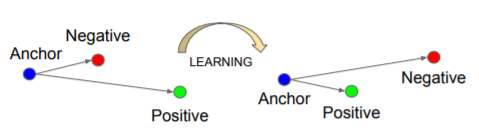
\includegraphics[width=0.5\textwidth]{figures/triplet_loss_figure}
        \caption{Diagram of the relative distances between triplet points. The distance between the anchor and the positive point should be minimized and the distance between the anchor and the negative point should be maximized. (Source: Schroff et al., 2015)}
        \label{Triplet Loss Diagram}
    \end{figure}
    
    N-pair loss (\cite{sohn2016improved}) extends on triplet loss to include more than one negative sample for each anchor and positive sample pairing. The authors write that by only comparing the anchor against one negative sample per loss computation, it takes much longer for the loss to converge. N-pair loss is especially useful for datasets in which there is more than two classes, as it is often the case that there are more negative samples than positive samples for each point. Consider a tuple of $N + 1$ elements consisting of an anchor point $x_{a}$, a positive sample $x_{p}$, and $n - 1$ negative samples $x_{n}^{1}, x_{n}^{2}, ..., x_{n}^{N - 1}$. We can then define the loss objective as follows.
    \begin{equation*}
    L_{\text{N-pairs}}(\theta, x_{a}, x_{p}, x_{n}^{1}, x_{n}^{2}, ..., x_{n}^{N - 1}) = log(1 + \sum_{i=1}^{N-1} 
    \exp(f_{\theta}(x)^{T} f_{\theta}(x_{n}^{i}) 
    - f_{\theta}(x)^{T} f_{\theta}(x_{p})
    )
    \end{equation*} 
    The N-pair loss differs from triplet loss not only in the use of multiple negative samples but primarily in it's use of the inner-product in the place of a distance metric.
    
    There are several general problems with contrastive approaches that have recently motivated research on alternative loss functions (\cite{hav4ik2021deepmetriclearning}). One of these issues is the computational complexity of sample mining. For most contrastive approaches (we will use triplet loss for this example) the most difficult triplets (in terms of minimizing the loss function) should be mined for the model to converge quickly. However, finding such triplets is often computationally expensive (\cite{hav4ik2021deepmetriclearning}). Another issue is that contrastive approaches  do not necessarily pull together objects of the same class to the same region of the latent space (\cite{hav4ik2021deepmetriclearning}). Both of these issues are addressed by more recent metric loss functions.
    
    \subsection{Modern Metric Losses}
    Modern metric loss functions address some of the shortcomings of traditional contrastive metric losses, such as supervised contrastive loss (\cite{khosla2020supervised}). Though originally proposed for a self-supervised learning problem, further generalizes triplet and N-pair loss by using many positive and many negative samples for each loss computation, which the authors attribute as the reason the loss is able to converge quickly without mining for hard samples. \\ 
    
    \begin{equation*}
    L_{out}^{sup} = \sum_{i \in I} \frac{-1}{|P(i)|}
    \sum_{p \in P(i)}log(\frac{\exp(z_{i} \cdot z_{p} / \tau)}
    {\sum_{a \in A(i)}\exp(z_{i} \cdot z_{a} / \tau)}) 
    \end{equation*} 
    \begin{equation*}
    L_{in}^{sup} = \sum_{i \in I} -log(\frac{1}{|P(i)|}\sum_{p \in P(i)}
    \frac{\exp(z_{i} \cdot z_{p} / \tau)}
    {\sum_{a \in A(i)}\exp(z_{i} \cdot z_{a} / \tau)}) 
    \end{equation*}
    
    The two implementations proposed in the paper differ only in taking the logarithm outside or inside the summation. In both equations, $I = {1, ..., 2N}$ is the set of indexes in the batch, $A(i) = I \setminus \{i\}$ is the set of indexes excluding $i$, $P(i) = \{p \in A(i) : y_{p} = y _{i}\}$ is the set of positive indexes in the batch for a given index $i$ excluding $i$ itself, and $\tau \in \mathbb{R}^{+}$ is a temperature hyperparameter. Like the N-pair loss, the supervised contrastive loss is modeled around the softmax loss. Unlike the N-pair loss, the supervised contrastive loss can be computed once per batch and includes multiple \textit{positive} samples in one computation. \\
    
    The center loss is another important modern metric loss in solving some of the problems with contrasting learning. (\cite{10.1007/978-3-319-46478-7_31}). To address the previously mentioned problem of latent points not self-organizing into regions based on class, the authors introduce a center loss $L_{C}$ to encourage a point of class $y_{i}$ to be close to the corresponding class center. The class center $c_{y_{i}}$ for class $y_{i}$ is a trainable parameter which updates with the overall loss function, which is stated below.
    \begin{equation*}
    L_{C} = \frac{1}{2}\sum_{i = 1}^{n}||x_{i} - c_{y_{i}}||_{2} \end{equation*}
    \begin{equation*}
    L_{S} = - \sum_{i = 1}^{n} g_{y_i}(x_i)
    \end{equation*}
    \begin{equation*}
    L = L_{S} + L_{C}
    \end{equation*}
    In the above equations, the center loss $L_{C}$ is added to a softmax loss $L_{S}$ in the overall loss function. $g_{c}$ refers to the softmax classification probability for class $c$, and $n$ is the number of elements in the batch. \\
    
    Center loss can be viewed as one of the first steps in many of today's state of the art metric learning objectives. The SphereFace loss (\cite{liu2017sphereface}) is largely a modification of center loss's softmax function. SphereFace normalizes the class centers to be points on a hypersphere which gurantees consistency for inter-class variability. This is accomplished through normalizing of each row of the weight's matrix in the softmax function such that the norm of the row vector is 1. SphereFace additionally adds a margin term such that the decision boundary between classification of a point with softmax is more robust.  Other State-of-the-Art metric losses, such as CosFace (\cite{wang2018cosface}), ArcFace (\cite{deng2019arcface}), and AdaCos (\cite{zhang2019adacos}) are largely inspired by SphereFace and further explore the idea of a margin term for a decision boundary in angular projection (\cite{hav4ik2021deepmetriclearning}). \\

\end{document}
